\section{Bramka logiczna OR}%Gilbert Guszcza
\label{sec:guszcza}

Grafika bramki logicznej OR (see Figure~\ref{fig:or}).

\begin{figure}[hthp] % pozycjonuje obrazek
    \centering
    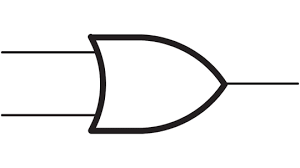
\includegraphics[width=0.2\textwidth]{pictures/OR.png} % Jak sprawić, żeby obrazek był większy?
    \caption{Bramka OR.}
    \label{fig:or}
\end{figure}

Tabloca~\ref{tab:OR} prawdy. % \ref odwołuje się do elementu po label

\begin{table}[htbp]
\centering
\begin{tabular}{|l|l|l|}
\hline
\rowcolor[HTML]{67FD9A} 
A & B & $A \vee B$ \\ \hline
0 & 0 & 0          \\ \hline
1 & 0 & 1          \\ \hline
0 & 1 & 1          \\ \hline
1 & 1 & 1          \\ \hline
\end{tabular}
\label{tab:OR}
\caption{Caption of my table is below it.}
\end{table}
\pagebreak
$$ det(A) = 0 \Leftarrow \exists_{i \in T} \exists_{z \in T } \quad  z \not= i \quad j \in T \quad a\in A \quad x \in F:$$$$a_{ij} = 0 \vee  a_{ji} = 0 \vee a_{zj} = x*a_{ij} \vee a_{jz} = x*a_{ji}$$
\begin{flushleft}
\underline{Lorem ipsum} dolor sit amet, consectetur adipiscing elit. Suspendisse pulvinar tincidunt magna eget vestibulum. Pellentesque sagittis, lectus at condimentum congue, lacus ligula aliquam nunc, viverra elementum justo enim vel est.    
\end{flushleft}
\begin{center}
\emph{Donec lacinia feugiat lorem, vel porta nisl volutpat aliquam. Pellentesque habitant morbi tristique senectus et netus et malesuada fames ac turpis egestas.}\par
Maecenas dapibus pellentesque tortor vitae maximus. Quisque sed malesuada purus. \textcolor{red}{Donec eu nisi commodo, egestas diam a, congue dolor.} Pellentesque porttitor, ex sed blandit bibendum, enim mauris aliquet felis, in pharetra nisi augue ac massa. Fusce tristique eros ullamcorper tempus varius. \textbf{In a efficitur sapien. Praesent quis consectetur mi.} Curabitur non mauris venenatis, pharetra ante nec, varius nunc. Phasellus dictum est nec elit tristique, id accumsan felis fermentum.
\end{center}

\begin{itemize}
  \item This is my first point
  \item Another point I want to make 
  \item[$\alpha$] Make the point fair and square.
  \item[NOTE] This entry has no bullet
  \item[] A blank label?
\end{itemize}
\vspace{5pt}
\begin{enumerate}
  \item This is my first point
  \item Another point I want to make 
\end{enumerate}
Tabloca~\ref{tab:OR} prawdy.